\chapter{Contexte du stage}
\label{AnalyseConception}

\section{Environnement de travail}

Durant le stage j'ai travaillé sur un pc de marque Dell, dont le système d'exploitation est Windows 8.1 Profesionnal (machine hôte). L'entreprise travaille avec de nombreuses machines virtuelles hébergées ou distantes afin de disposer d'environnement de tests, de développements, et de production. Pour cela, j'avais à ma disposition une machine virtuelle de développement via VirtualBox avec le système d'exploitation Windows Server 2012 R2 Standard. \\

\section{Outils utilisés}

Quotidiennement j'ai utilisé 2 environnements de développement intégré (IDE) : Liclipse (pour développer en langage Python) dans le projet DataWizard, et \textbf{Eclipse} version Mars (pour développer en langage Java/Java EE) pour les projets MobiSAAS et Crislab.\\

Dans les projets plusieurs \textbf{SGBD} sont manipulés : MongoDB (MobiSAAS), Oracle (Crislab), mais j'ai principalement travaillé avec \textbf{Postgresql} afin de gérer les données de mon module. De plus, Postgresql permet de gérer les données géographiques dans le projet "DataWizard" grâce à sa cartouche spatiale /\textbf{Postgis}.\\

Afin de tester les web services REST développés, j'ai utilisé fréquemment l'outil \textbf{SoapUI} (Fig. \ref{SoapUIGet}). Il permet de mettre en place une suite de tests qui peuvent être lancé d'une traite du côté client, permet de tester les services web en mode bouchon mais aussi d'effectuer des tests de charge. Il permet entre autre de fournir une hiérarchie des services web, de lister les différentes méthodes disponible, les paramètres attendus, de réaliser des requêtes et de récupérer les réponses … C'est l'un des meilleurs outils de test unitaires concernant les services web.

\begin{center}
\begin{figure}[h] \centering
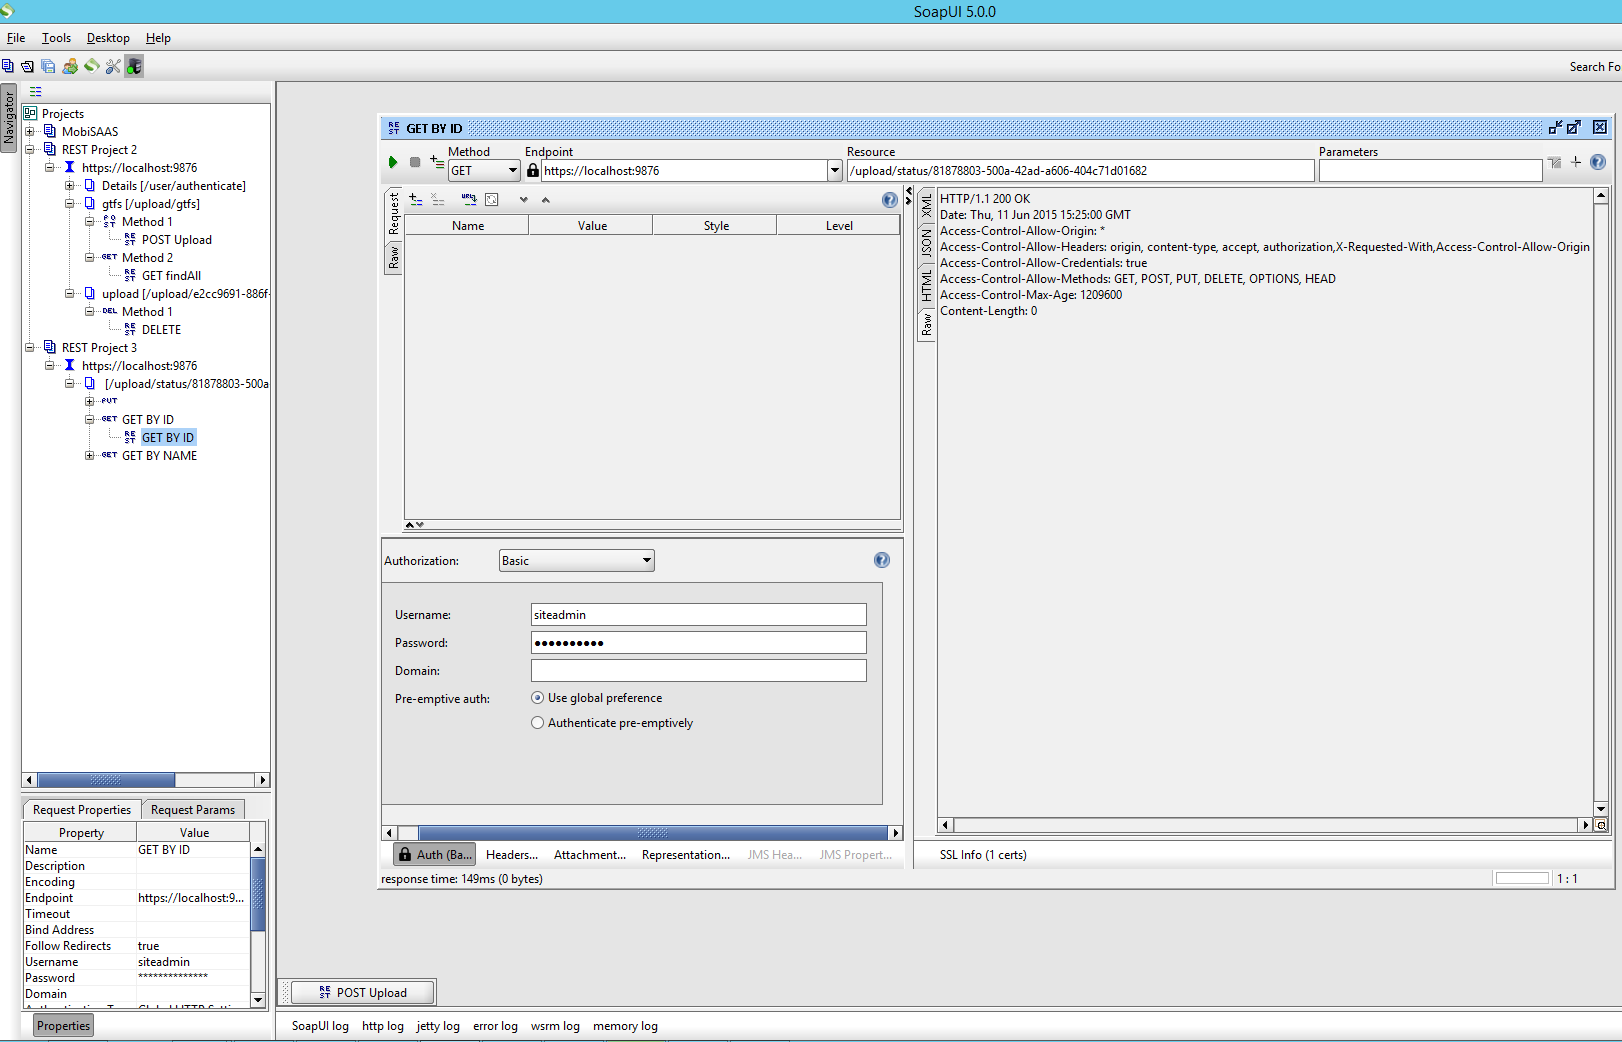
\includegraphics[width=16cm]{images/soapUI_getById_sansResponse_small.png}\\
\caption{\label{SoapUIGet} Interface et exemple de requête "GET" SoapUI}
\end{figure}
\end{center}


\section{Gestion de projets}

Dans les projets auxquels j'ai participé, l'entreprise utilise des outils de gestion : planning, suivi de bugs, outils de mutualisation, gestion de versions. Ainsi, j'ai utilisé l'outil Trello pour la gestion des tâches, Redmine pour la gestion des projets (cf. Annexe \ref{Annexe A}), et \textbf{SVN} pour la gestion des codes sources. L'entreprise met à disposition de ses salariés un intranet avec de nombreux outils collaboratifs sous la plateforme eGroupware (Feuille de temps,etc...).\\

J'ai effectué mon travail en étroite relation avec le chef de projet. A partir des spécifications techniques et fonctionnelles, les développements ont progressé et évolué tout le long de la période de réalisation. Sans pour autant pratiquer une méthode «Agile» au sens strict, plusieurs ajustements (mode itératif) ont été effectués et le dialogue quotidien à permis de toujours rendre mon travail en adéquation aux besoins. \\

Un point de suivi informel était effectué plusieurs fois par semaine avec mon responsable afin de présenter le travail effectué, les résultats intermédiaires, et le travail planifié pour la semaine suivante. Un bilan à la mi-stage a été effectué afin de réajuster les priorités, et arriver à produire un livrable satisfaisant en fin de stage. \\


\section{Difficultés rencontrées}

Il y a peu à dire, l'environnement "équipe" et les compétences de chacun ont été propices à les éviter. En effet, j'avais de chaque côté de mon bureau les 2 personnes les plus à même de débloquer des situations, ou me renseigner sur une question. Pour le projet MobiSAAS, j'ai eu des "difficultés" qui sont communes à chaque évolution de version d'un framework. En effet, au milieu du stage il a fallu "recoder" dans plusieurs parties du code pour s'adapter aux évolutions lors du passage de la version 0.7.1 à la version 0.8.1 de Dropwizard.
Sinon, pour le projet DataWizard et d'une manière générale, une des difficulté a été de répondre aux experts et analystes en réseaux de transport et produire des résultats (Métadonnées, Rapport JSON, etc...) exploitables et conformes à leurs attentes. Cela a demandé du dialogue et de se mettre en accord sur la terminologie à employer (ex: EdgeType, PTMode,...). Tous ces termes courants pour les experts ne sont pas intuitifs pour les développeurs... Encore une fois, je pense que cet aspect "métier" qui demande de l'adaptation est commun à tous les projets.\\
